\documentclass{./acm_proc_article-sp}

\begin{document}

\title{Procedural Content Generation for Computer Games}
\subtitle{A survey of techniques used for procedural content generation for computer games, classified by beneficiary.}

\numberofauthors{1}
\author{
\alignauthor
Thomas Smith\\
       \affaddr{Electronics and Computer Science}\\
       \affaddr{University of Southampton}\\
       \email{taes1g09@ecs.soton.ac.uk}
}

\maketitle
\begin{abstract}
Modern computer games make use of a wide variety of procedural content generation (PCG) techniques that serve a number of purposes during the development of a game. Though PCG techniques have been used since some of the earliest computer games\cite{elite}, they are now becoming increasing relevant as AAA games become larger and more detailed and indie games teams become smaller. PCG techniques can easily amplify production efforts by automating asset generation or augmenting manual content production, and they can be a powerful tool to allow developers to create and populate varied and believable playspaces. They can also play a role in customising each player's experience to improve engagement and entertainment. This paper provides a high-level classification of a range of techniques used for different types of content, and attempts to discern common aspects and transferable approaches that can help to promote a more unified, standard approach to content generation for games. 


% Improve variety, allow developers to populate large areas, allow customisation to player preferences, reduce assets, allow control/tweaking, reduce labor costs
% algorithmic generators rather than manual construction. 
% incentive to automate the production of material
% specialised techniques, each tailored to a particular kind of content
% concepts from AI used to improve the quality and relevance of the generated content
% intelligently breeding possibilities from a population of solutions or applying machine learning to create a map between player behaviour and optimal content. 
% Each genre of game and each kind of generated content has a range of potential techniques that may be useful for its production, 
% each game requires different content
% there are not yet standard approaches to integrating multiple kinds of content generation.



% Hundreds of millions of people play computer games every day. For them, game content–from 3D objects to abstract puzzles– plays a major entertainment role. Manual labor has so far ensured that the quality and quantity of game content matched the demands of the playing community, but is facing new scalability challenges due to the exponential growth over the last decade of both the gamer population and the production costs. Procedural Content Generation for Games (PCG-G) may address these challenges by automating, or aiding in, game content generation. PCG-G is difficult, since the generator has to create the content, satisfy constraints imposed by the artist, and return interesting instances for gamers. Despite a large body of research focusing on PCG-G, particularly over the past decade, ours is the first comprehensive survey of the field of PCG-G. We first introduce a comprehensive, six-layered taxonomy of game content: bits, space, systems, scenarios, design, and derived. Second, we survey the methods used across the whole field of PCG-G from a large research body. Third, we map PCG-G methods to game content layers; it turns out that many of the methods used to generate game content from one layer can be used to generate content from another. We also survey the use of methods in practice, that is, in commercial or prototype games. Fourth and last, we discuss several directions for future research in PCG-G, which we believe deserve close attention in the near future.
\end{abstract}

% A category with the (minimum) three required fields
% \category{H.4}{Information Systems Applications}{Miscellaneous}
%A category including the fourth, optional field follows...
% \category{D.2.8}{Software Engineering}{Metrics}[complexity measures, performance measures]

% \terms{Theory}

% \keywords{ACM proceedings, \LaTeX, text tagging} % NOT required for Proceedings

\section{Introduction}
Intoduction to the topic, explanation of lack of structure. Reference to the age of things, Elite\cite{elite}, nethack, increasing use in successful commercial games. The need for procedural content generation.

\subsection{Background}
Building on the work of Hendrikx et. al \cite{hendrikx2012procedural} this paper provides a modern overview of the range of procedural content generation techniques used in games today.
\subsection{Methodology}
Given the broad range of procedural content techniques, this review organises approaches first by the primary user of each method. Lists a number of the main purposes that PCG is used for within that category, along with examples and academic literature in that area.


\section{Artists}
%methods and results
When producing the raw content that goes into a game, procedural generation techniques can provide a more efficient method or greater variety than building everything by hand. Many of these techniques are not unique to the field of computer games and are also used to produce computer-generated graphics for all kinds of media, from animated movies to photorealistic bcakgrounds in advertisements and print media.

\subsubsection{Textures}

Perlin Noise
Grammars
Long history of using perlin noise effects for material textures. Originally developed by Ken Perlin in <year>, it provides <definition>. Used for everything from clouds to marble.
Pattern-based textures. Ideal for providing high-resolution texturing across large landscapes. Algorithmically generates textures with specified features, useful for either repetetive applications such as hich-rise city blocks or aperiodic such as natural landscapes \cite{patternTextures}
\subsubsection{Models}
visual variety, procedural construction
fill space - speedtree\cite{speedtree}, procedural cities
Borderland's guns
Grammars
Speedtree
\subsubsection{Animation}
Rather than create animations for all possibilites (counterexample - assassins creed 3 had <number> of distinct animations)
Respond to conditions that weren't known at design time: user content generation - Spore\cite{Spore}, allows charaters to react to a vast range of physical conditions - Jedi Unleashed force push, Emotion engine.
\subsubsection{Effects}
Procedural generation of environmental effects such as fire, water, smoke and clouds. Provides believable variety (starter point for citations in \cite{hendrikx2012procedural})
Particles
Generation of effects representing spells and weapons allows customisation based upon the properties of the ability \cite{particles}
Procedural rendering effects - allows graphical styles that are radically distinct from traditional photorealistic techniques \cite{kowalski1999art}
\subsubsection{Music}
Allows great variety - specify a style, and get infinite variations. \cite{collins2009introduction} <Does this belong in designers? often reacts to in-games event, used to build mood>

%comparison and evaluation of approaches
\subsection{Benefits}
Two of the main benefits associated with artists' use of PCG techniques are the reduction in labor required to make a large variety of variations on a them, and the reduced storage requirement to represent this variets. This is becoming increasingly relevant as games become larger and the status quo shifts from physical to digital distribution - smaller games means faster delivery
Download sizes - procedural variation - Borderland's enemies
\subsubsection{Future work}

\section{Designers}
%methods and results

\subsection{Varieties}
\subsubsection{Content scale}
Use of PCG allows designers to populate large game spaces with a high level of detail and variety. Middleware packages such as Speedtree\cite{speedtree} allow entire forests to be generated and customised, and similar approaches exist for generating believable cities and landscapes.

\subsubsection{Replayability}
The use of <semi-random> techniques means that play-spaces genearted using PCG may be different for each player, and for each player's playthrough of a game. The variety ensures that content is fresh each time, and minimises the effects of repetition - players are not able to memorise the precise route through each dungeon and locations of treasures, and so there is a sense of diecovery and exploration each time.

\subsubsection{Challenge}
On of the main factors that affects players' enjoment of games is their ability to remain in a state of `flow' - the sensation that their abilities are matched to the challenge provided by the game\cite{flow}.
In order to cater to the wide range in ability of players that each game may attract, many games have previously offered the option of customising the challenge experienced to one of a number of pre-set `difficulty levels'. <Read through 3yp for citations on difficulties with self-assessment and mutability>. Rather than <set> the degree of challenge at design time, Lopes et al. show that it is possible to adaptively generate or alter aspects of the game\cite{lopes2011adaptivity} in order to match the observed ability of the player\cite{ResE5}.

%comparison and evaluation of approaches
\subsection{Benefits}
Speed up work - large, beliveable diverse playspaces\\
close the gap between designer and player - allow modification based on individual information about the player.
\subsubsection{Future work}
Improve automated critics \cite{hendrikx2012procedural}

\section{Users}
%methods and results

\subsubsection{Experience}
Valve's AI Director
Bethesda's Radiant Storytelling
\subsubsection{Agency}
Typically, no direct player control over adaptive generation (cite hamlet)
however, in some games that make use of procedural generation it can be a benefit to give the player some degree of direct control over the generation process - for example a recent addition to the GAR was the `'Weapons Lab', a portion of the game where players may spend in-game resources to customise their procedurally-generated weapons. (cite GAR's weapons lab)
Radiant Story?
GAR's weapons

%comparison and evaluation of approaches
\subsection{Benefits}
Users get a more engaging experience that can be tailored specifically to their preferences and abilities
\subsubsection{Future work}
% player control over procedural content generation

\section{Conclusion}
% a comparison and evaluation of approaches, and an indication of the outstanding, unsolved, issues and problems.
We can see that a variety of <stakeholders> benefit from the improvement of procedural content techniques, and that there are a wide range of existing techniques used for a plethora of different reasons.

%ACKNOWLEDGMENTS are optional
% \section{Acknowledgments}

\bibliographystyle{abbrv}
\bibliography{draft}
%\balancecolumns
% \appendix
% \section{Project Brief}
\begin{figure*}
\centering
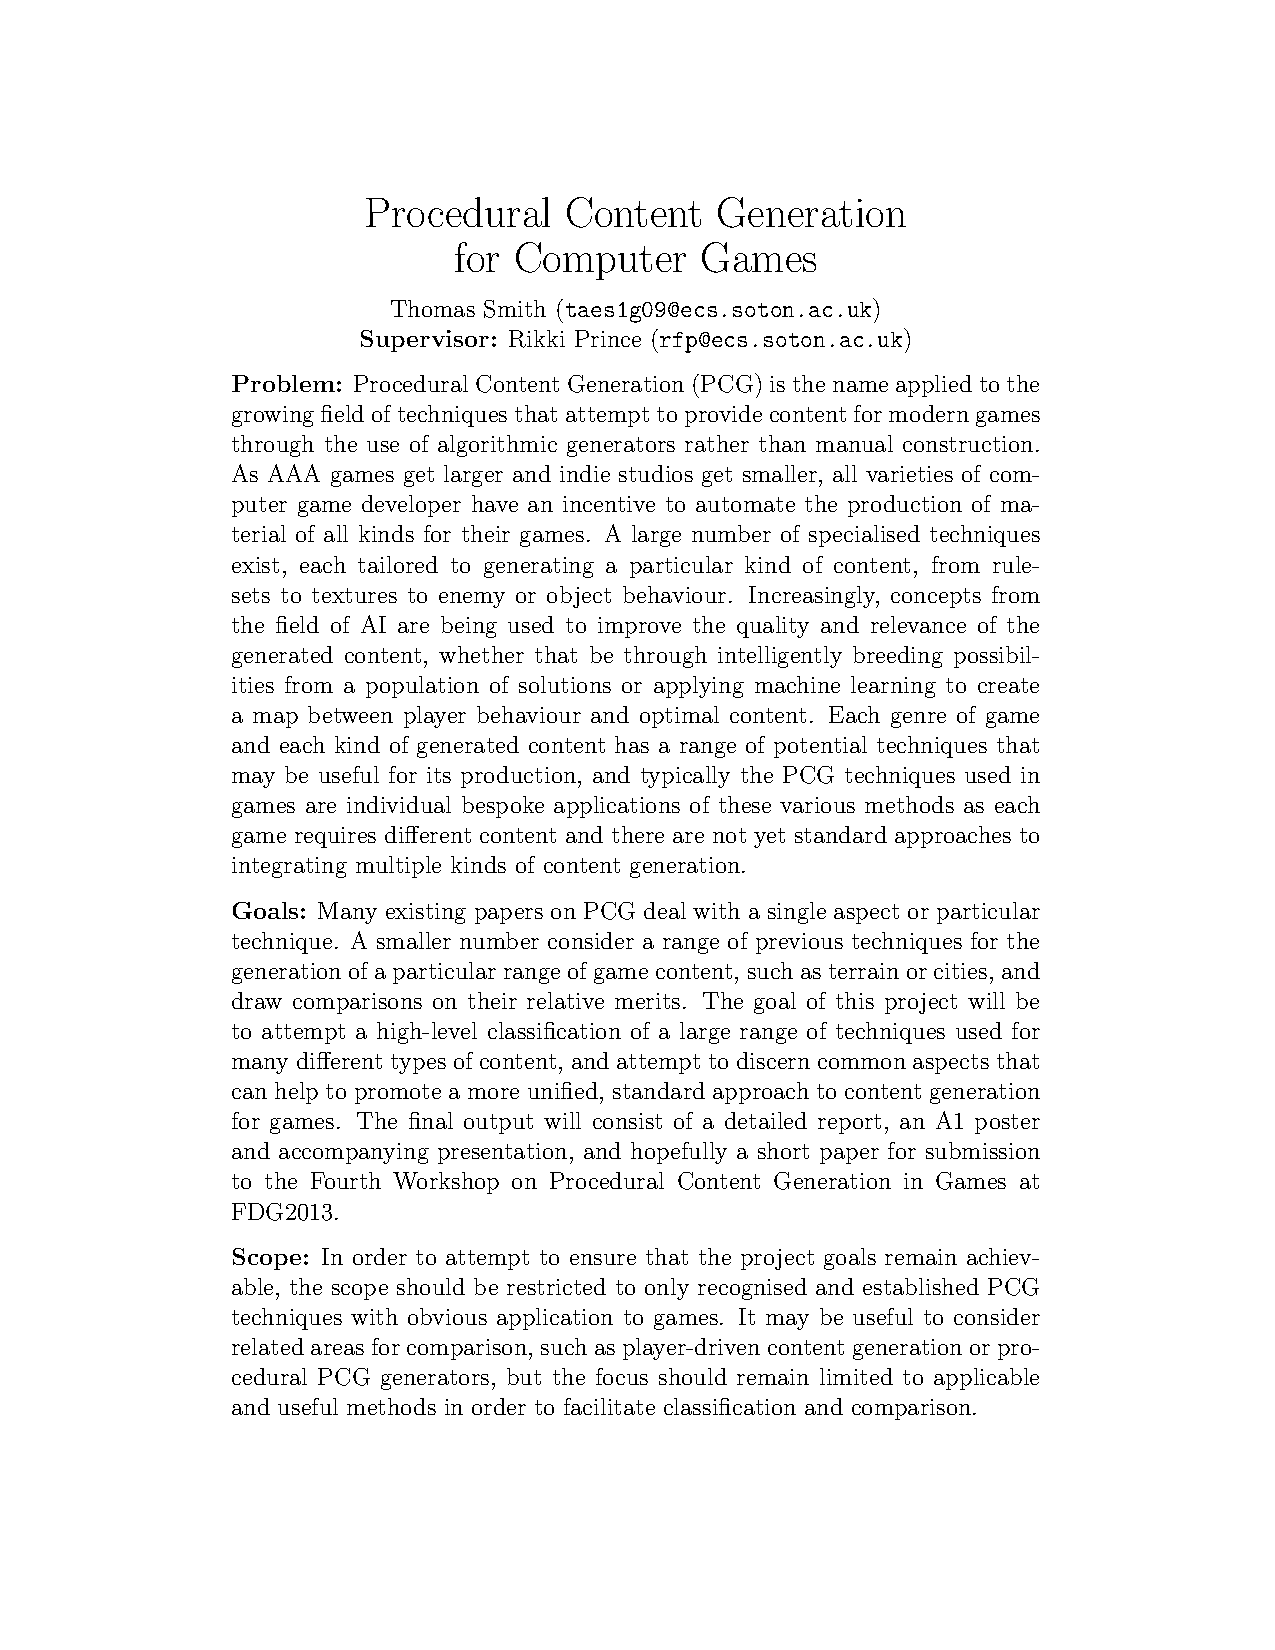
\includegraphics{../Brief/Project Brief.pdf}[clip trim=200 200 200 200]
\end{figure*}
\balancecolumns
% That's all folks!
\end{document}

You should read and summarise these articles, producing a 8 page, using a two-column format, survey article indicating the background to the problem, the methods and results presented in your group of articles, a comparison and evaluation of approaches, and an indication of the outstanding, unsolved, issues and problems.
